\documentclass{resume} % Use the custom resume.cls style

\usepackage[left=0.75in,top=0.6in,right=0.75in,bottom=0.6in]{geometry} % Document margins
\usepackage{xcolor}
\usepackage{hyperref}
\hypersetup{
    colorlinks=true,
    linkcolor=blue,
    filecolor=magenta,      
    urlcolor=teal,
}
\usepackage{graphicx}
\newcommand{\tab}[1]{\hspace{.2667\textwidth}\rlap{#1}}
\newcommand{\itab}[1]{\hspace{0em}\rlap{#1}}
\name{Emilio Berti} % Your name
\address{
    \centering
    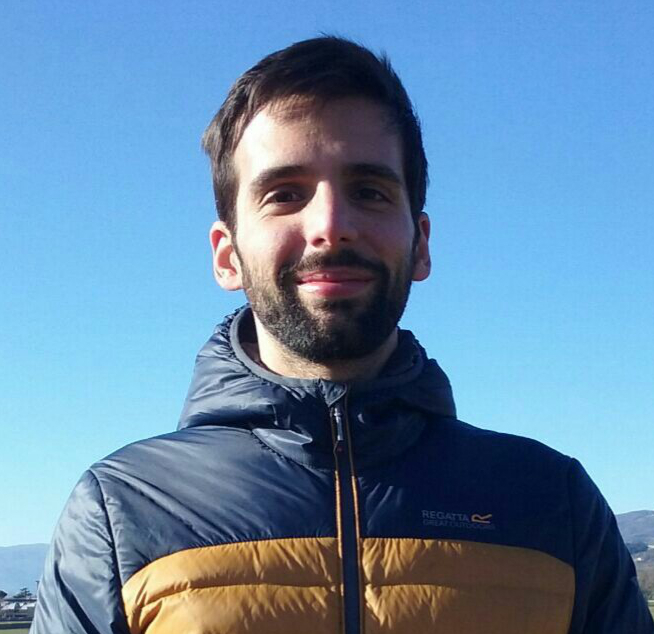
\includegraphics[width=0.30\textwidth]{Emilio.jpg}
}
\address{(+45) 266 54 662 \\ emilio.berti.academia@gmail.com}

\begin{document}

\begin{rSection}{Summary}
I am a theoretical ecologist with a passion for math and computing.
I have an strong quantitative background, with expertise in mathematical and statistical modelling of complex systems using big databases at large spatio-temporal scales.
I have worked in many different fields of biology, from molecular muscle physiology to macroecology and biogeography.
I am a very quantitative person, with a wide, in-depth understanding of traditional as well as cutting-edge statistical approaches.
Currently, my main research interests lie in the intersection between climate science and theoretical community ecology, e.g. understanding the climatic, environmental, and biotic drivers of biodiversity.
I enjoy programming very much; I started by prototyping robots and I haven't stop since.
I have outstanding programming skills in several languages, particularly in R, python, and C++, and a strong background in Geographic Information Systems (GIS), especially in optimizing large computations and performing complex data analyses on high-performance clusters.
This, together with my very collaborative personality, helped me establish long-term collaborations in several institutions, mostly in Denmark, Germany, and Italy.

\end{rSection}

\begin{rSection}{Work History}

{\bf PostDoctoral researcher} \hfill {\em October 2020 -- Present}\\
Theory in Biodiversity Science\\
German Centre for Integrative Biodiversity Research (\textsc{iDiv})\\
Leipzig, Germany

{\bf Scientific consultant} \hfill {\em May 2020 -- July 2020}\\
Department of Bioscience\\
Aarhus University\\
Aarhus, Denmark

{\bf Teaching assistant} \hfill {\em February 2017 -- April 2020}
\\Department of Biology\\
Aarhus University\\
Aarhus, Denmark

\end{rSection}

\begin{rSection}{Education}
{\bf PhD} \hfill {\em February 2017 -- June 2020} 
\\ Section of Ecoinformatics and Biodiversity
\\ Department of Biology
\\ Aarhus University
\\ Aarhus, Denmark
\clearpage
{\bf Visiting PhD student} \hfill {\em Fall 2018}
\\ Department of Ecology and Evolution
\\ University of Chicago
\\ Chicago, IL

{\bf MSc in Biology} \hfill {\em 2013 -- 2016}
\\ Department of Ecology and Evolution
\\ University of Florence
\\ Florence, Italy

{\bf BSc in Biology} \hfill {\em 2009 -- 2012}
\\ Department of Physiology
\\ University of Florence
\\ Florence, Italy
\vskip3ex
\end{rSection}

\begin{rSection}{Postgraduate courses}
{\bf ``Species Distributions Modelling''} \hfill {\em 2019}\\
Evora, Portugal -- Lecturers: Prof. Miguel Ara\'{u}jo and Dr. Babak Naimi\\
{\bf ``Megafauna ecology -- shaping past, present and future ecosystems.''} \hfill {\em 2019}\\
Aarhus, Denmark\\
{\bf ``Mixed models''} \hfill {\em 2019}\\
Aarhus, Denmark -- Lecturer: Prof. Rodrigo Labouriau\\
{\bf ``Writing and Speaking Science in English for Biology Students''} \hfill {\em 2019} \\
Aarhus, Denmark -- Lecturer: Prof. Brian Sorrell \\
{\bf ``Ecosystem roles of megafauna in the past, present, and future''} \hfill {\em 2017}\\
Aarhus, Denmark\\
{\bf ``Mediterranean School of Complex Networks (MSCx)''} \hfill {\em 2017} \\
Salina, Italy
\end{rSection}

\begin{rSection}{Skills}
{\bf Language}\\
Italian (native), English (fluent), Danish (beginner), German (beginner)\\
{\bf Programming}\\
R (expert), python (expert), bash (expert), C/C++ (proficient), javascript (mostly for Google Earth Engine, proficient), SQL (postgres flavour, proficient), html (proficient), High Performance Computing (HPC SLURM flavour, expert)\\
{\bf Software} \\
Linux/GNU, Anaconda, QGIS, \LaTeX, Markdown, Pandoc, Git, GitHub, ssh\\
{\bf Methods} \\
Statistics, regression analysis, effect sizes, mixed models, variables selection, PCA, ordination and classification, optimization, machine learning, network analysis, mathematical modelling, data science, extrapolation and forecasting, species distribution models, climate analyses, environmental niche modeling, spatial modeling, geographic information systems (GIS), demographic projections, biodiversity/climate models, big data, data visualization, high-performance clusters, automation.
\end{rSection}

\begin{rSection}{Teaching \& Organized Workshops}
{\bf Teaching} \\
Introduction to scientific programming and tidyverse (2022) -- \href{https://emilio-berti.github.io/teaching/tidyverse.html#(1)}{slides}\\
Introduction to git and GitHub for a fool-proof programming (2022) -- \href{https://emilio-berti.github.io/idiv-git-introduction/}{course}\\
\clearpage
{\bf Teaching Assistant} \\
Meta-analyses for Biodiversity (2021)\\
Statistical and Geospatial Modelling (2019)\\
Behavioural Biology (2018, 2019)\\
Geographic Information System (2017)\\
{\bf Organized Workshops}\\
Cleaning online repository data for use in biogeography and macroecology (2019)\\
Running a species distribution model in R (2019)\\
A (very) gentle introduction to Linux (2019)
\end{rSection}

% \begin{rSection}{References}
% \textbf{Jens-Christian Svenning} (Professor)\\
% Aarhus University, Department of Biology, Ecoinformatics and Biodiversity\\
% E-mail: svenning@bios.au.dk
% Phone: +45 289 92 304

% \textbf{Robert Buitenwerf} (Assistant Professor)\\
% Aarhus University, Department of Biology, Ecoinformatics and Biodiversity\\
% E-mail: buitenwerf@bios.au.dk\\
% Phone: +45 871 54 346

% \textbf{Giacomo Santini} (Assistant Professor)\\
% Florence University, Department of Biology\\
% E-mail: giacomo.santini@unifi.it\\
% Phone: +39 055 45 74 721
% \end{rSection}

\begin{rSection}{Publications}
% \vspace{4ex}\hfill{\em 2020}\\
Gauzens, B., Brose, U., Delmas, E., \& \textbf{Berti, E}. (2023). ATNr: Allometric Trophic Network models in R. Methods in Ecology and Evolution.

Wei, S., \textbf{Berti, E.}, ... \& Yue, K. (2023). Global patterns and drivers of lead concentration in inland waters. Journal of Hazardous Materials, 132455.

Dyer, A., Brose, U., \textbf{Berti, E.}, Rosenbaum, B., \& Hirt, M. (2023). Heat dissipation drives the hump-shaped scaling of animal dispersal speed with body mass. bioRxiv. (Accepted in Plos One).

Terlau, J., Brose, U., Antunes, A. C., \textbf{Berti, E.}, Boy, T., Gauzens, B., ... \& Hirt, M. R. (2022). Integrating trait-based movement into mechanistic predictions of thermal performance.

Bauer, B., \textbf{Berti, E.}, ... \& Brose, U. (2022). Biotic filtering by species’ interactions constrains food-web variability across spatial and abiotic gradients. \textit{Ecology letters}. DOI: \href{https://doi.org/10.1111/ele.13995}{10.1111/ele.13995}. (\texttt{Shared first authorship}).

Grenié, M, \textbf{Berti, E.}, ... \& Marten, W. (2022). Harmonizing taxon names in biodiversity data: a review of tools, databases, and best practices. \textit{Methods in Ecology and Evolution}. DOI: \href{https://doi.org/10.1111/2041-210X.13802}{10.1111/2041-210X.13802}.

\textbf{Berti, E.}, Davoli, M., ... \& Vollrath, F. (2021). The r package enerscape: A general energy landscape framework for terrestrial movement ecology. \textit{Methods in Ecology and Evolution}. DOI: \href{https://doi.org/10.1111/2041-210X.13734}{10.1111/2041-210X.13734}.

\textbf{Berti, E.}, Monsarrat, S., Munk, M., Jarvie, S. \& Svenning, J.C. (2020). Body size is a good proxy for vertebrate charisma. \textit{Biological Conservation}. DOI: \href{https://doi.org/10.1016/j.biocon.2020.108790}{10.1016/j.biocon.2020.108790}.

\textbf{Berti, E.} \& Svenning, J.C. (2020). Megafauna extinctions have reduced biotic connectivity worldwide. \textit{Global Ecology and Biogeography}. DOI: \href{https://doi.org/10.1111/geb.13182}{10.1111/geb.13182}.
\end{rSection}

\begin{rSection}{Conference talks}
Bauer, B., \textbf{Berti, E.}, \dots, \& Brose, U. (2022). From regional to local scale: biotic interactions shape multilayer food-webs. \textit{SFE-GFO-EEF biannual meeting, Metz, France}

\textbf{Berti, E.}, \& Svenning, J.C. (2022). State-space models show that functional replacements of extinct megafauna have distinct habitat preference in a European rewilding area. \textit{SFE-GFO-EEF biannual meeting, Metz, France}

Grenié, M., \textbf{Berti, E.}, Carvajal-Quintero, J., Winter, M., \& Sagouis (2021). Matching Species Names Across Biodiversity Databases: Sources, tools, pitfalls and best practices for taxonomic harmonization. \textit{TDWG annual meeting, online}

\textbf{Berti, E.} \& Svenning, J.C. (2019). Megalinkers extinction and the decrease of ecosystem connectivity. \textit{ESA annual meeting, Louisville, KY}

\textbf{Berti, E.}, Jarvie, S. W., \& Svenning, J.C. (2018). Rewiring food webs via trophic rewilding. \textit{BES annual meeting, Belfast, UK}
\end{rSection}

\begin{rSection}{Peer review}
As of July 2022, I have reviewed 6 papers for: Ecography (2), Ecology Letters (2), GigaScience (1), and Scientia Agricola (1). You can find more at my \href{https://publons.com/wos-op/researcher/4208953/emilio-berti/}{Publons profile}.
\end{rSection}

\begin{rSection}{Links}
\begin{minipage}{0.5\textwidth}
\begin{itemize}
    \item \href{https://scholar.google.com/citations?user=5KPh-oUAAAAJ&hl=en}{Google Scholar profile}
    \item \href{https://emilio-berti.github.io/}{Personal website}
    \item \href{https://orcid.org/0000-0001-9286-011X}{ORCiD}
\end{itemize}
\end{minipage}
\begin{minipage}{0.5\textwidth}
\begin{itemize}
    \item \href{https://www.linkedin.com/in/emilio-berti-55a348146}{LinkedIn}
    \item \href{https://github.com/emilio-berti}{GitHub}
    \item \href{https://publons.com/wos-op/researcher/4208953/emilio-berti/peer-review/}{Publons}
\end{itemize}
\end{minipage}
\end{rSection}

\end{document}
